\subsection{Cattura elettronica}

Nel processo di cattura elettronica nel \na{}
viene emesso solo il fotone del neon a \SI{1275}{keV} e non il positrone.
Vogliamo misurare il rapporto di decadimento della cattura elettronica.
Le uniche informazioni precise sui rate parziali le possiamo estrarre dai fotopicchi
perché sono le uniche parti dello spettro che distinguiamo chiaramente
e per le quali abbiamo un modello ragionevole (la gaussiana).

\subsubsection{Normalizzazione del rate}

L'ADC riesce a leggere solo una frazione degli eventi,
però è ragionevole supporre che la decimazione sia imparziale,
quindi per ottenere il rate parziale di una regione dello spettro
basta moltiplicare il numero di eventi in quella regione
per il rate misurato dal contatore
e dividere per il numero totale di eventi registrati dall'ADC.

\subsubsection{Fotopicchi}

\begin{figure}
	\centering
	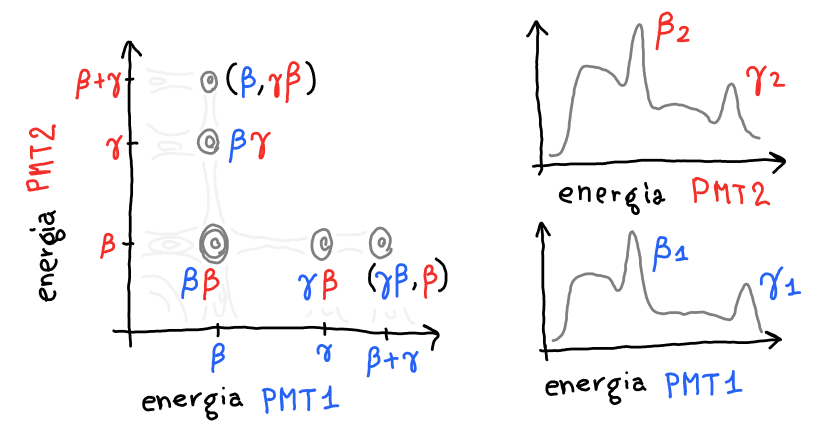
\includegraphics[width=27em]{immagini/schemapicchi}
	\caption{\label{fig:schemapicchi}
	Schema dei fotopicchi usati per misurare il branching ratio di cattura elettronica della sorgente \na{}.
	$\beta$ sono i fotoni emessi dall'annichilazione dei positroni
	e $\gamma$ quelli emessi dal neon eccitato in cui decade il \na.}
\end{figure}

Usando due scintillatori\footnote{Non abbiamo considerato configurazioni con tre rivelatori per questa misura.} possiamo ricavare il rate di undici fotopicchi diversi,
corrispodenti alle varie configurazioni con cui i fotoni possono interagire con i rivelatori;
di questi undici ne useremo però al più nove,
riportati schematicamente in \autoref{fig:schemapicchi}.
Indichiamo con $\beta$ i fotoni di annichilazione (\SI{511}{keV})
e con $\gamma$ i fotoni del neon (\SI{1275}{keV}).
Chiamiamo i rivelatori ``1'' e ``2''.
Cinque fotopicchi si ottengono dalle coincidenze a due:
\begin{description}
	\item[$\beta\beta$:]
	Caso in cui entrambi i rivelatori vedono i fotoni di annichilazione contrapposti e li assorbono.
	Questo picco è presente solo se la sorgente è tra i due rivelatori.
	\item[$\gamma\beta$:]
	Caso in cui il rivelatore 1 assorbe il fotone $\gamma$ e il 2 uno dei $\beta$.
	\item[$\beta\gamma$:]
	Come $\gamma\beta$ ma con $\beta$ sul rivelatore 1 e $\gamma$ sul 2.
	\item[$(\beta,\gamma\beta)$:]
	Il rivelatore 1 assorbe $\beta$ e il rivelatore 2 assorbe l'altro $\beta$ e $\gamma$.
	Come $\beta\beta$, questo segnale è presente solo se la sorgente si trova interposta tra i rivelatori.
	\item[$(\gamma\beta,\beta)$:]
	Come il precedente ma con i rivelatori scambiati di ruolo.
\end{description}
Gli altri quattro fotopicchi si ottengono triggerando su uno scintillatore alla volta:
per ogni scintillatore di ottiene un picco $\beta$ e un $\gamma$,
distinguiamo i rivelatori con un pedice: $\beta_1$, $\gamma_1$, $\beta_2$, $\gamma_2$.

\subsubsection{Equazioni dei rate}
\label{sec:eqrate}

Per ogni fotopicco misuriamo il rate.
Scrivendo i rate in funzione delle efficienze e accettanze dei rivelatori
e in funzione del rate di $\beta$ e del rate di $\gamma$
(diversi perché c'è la cattura elettronica)
otteniamo un sistema di equazioni da cui dobbiamo ricavare i rate.
Poiché in generale l'accettanza e l'efficienza non sono fattorizzate, le teniamo combinate.
Usiamo le variabili:
\newcommand*\tot{^\text{tot}}
\newcommand*\R{r}
\newcommand*\Rtot{\mathcal{R}}
\begin{description}
	\item[$\R$:]
	Rate $\beta$.
	\item[$\Rtot$:]
	Rate $\gamma$, ovvero $r$ più il rate di cattura elettronica.
	\item[$p_{\beta1}$, $p_{\beta2}$, $p_{\gamma1}$, $p_{\gamma2}$:]
	Probabilità di assorbimento per i vari fotoni/rivelatori.
	\item[$p_{\beta12}$:]
	Probabilità di assorbimento in coincidenza dei due fotoni $\beta$.
	\item[$p_{\beta1}^\text{tot}$, $p_{\beta2}^\text{tot}$, $p_{\gamma1}^\text{tot}$, $p_{\gamma2}^\text{tot}$:]
	Probabilità di rivelazione totali per i vari fotoni/rivelatori,
	cioè in pratica, rispetto alle variabili senza apice, è incluso il caso in cui il fotone fa Compton.
	\item[$p_{\beta12}^\text{tot}$:]
	Probabilità di rivelazione totale per i fotoni in coincidenza
	\emph{con l'esclusione del caso in cui fanno entrambi Compton}.
	\item[$R_{\beta1}$, $R_{\beta2}$, $R_{\gamma1}$, $R_{\gamma2}$, $R_{\beta\beta}$, $R_{\gamma\beta}$, $R_{\beta\gamma}$, $R_{\beta,\gamma\beta}$, $R_{\gamma\beta,\beta}$:]
	Rate dei vari fotopicchi.
\end{description}
Le equazioni sono
\begin{align}
	R_{\beta\beta} \label{eq:betabeta}
	&= \R p_{\beta12} (1 - p_{\gamma1}\tot - p_{\gamma2}\tot) \\
	R_{\gamma\beta} \label{eq:gammabeta}
	&= 2\R p_{\beta2} p_{\gamma1} - \R p_{\beta12}\tot p_{\gamma1} \\
	R_{\beta\gamma} \label{eq:betagamma}
	&= 2\R p_{\beta1} p_{\gamma2} - \R p_{\beta12}\tot p_{\gamma2} \\
	R_{\beta,\gamma\beta} \label{eq:betagammabeta}
	&= \R p_{\beta12} p_{\gamma2} \\
	R_{\gamma\beta,\beta} \label{eq:gammabetabeta}
	&= \R p_{\beta12} p_{\gamma1} \\
	R_{\beta1}
	&= 2\R p_{\beta1} (1 - p_{\gamma1}\tot) \\
	R_{\gamma1} \label{eq:gamma1}
	&= p_{\gamma1}(\Rtot - 2 \R p_{\beta1}\tot) \\
	R_{\beta1}
	&= 2\R p_{\beta2} (1 - p_{\gamma2}\tot) \\
	R_{\gamma2} \label{eq:gamma2}
	&= p_{\gamma2} (\Rtot  - 2 \R p_{\beta2}\tot).
\end{align}
Nel caso in cui la sorgente non sia interposta tra i rivelatori
bisogna eliminare le equazioni \eqref{eq:betabeta}, \eqref{eq:betagammabeta}, \eqref{eq:gammabetabeta}
e porre $p_{\beta12}\tot = 0$ in \eqref{eq:gammabeta} e \eqref{eq:betagamma}.

Notiamo che $\Rtot$ compare solo nelle equazioni \eqref{eq:gamma1} e \eqref{eq:gamma2}.
Notiamo anche che $\R$ compare solo a moltiplicare le variabili
$p_{\beta1}$, $p_{\beta2}$, $p_{\beta12}$, $p_{\beta1}\tot$, $p_{\beta2}\tot$, $p_{\beta12}\tot$
e che, viceversa, queste compaiono solo a moltiplicare $\R$,
cioè questo insieme di 7 variabili è degenere e va ridotto alle 6 variabili
$\R p_{\beta1}$, $\R p_{\beta2}$, $\R p_{\beta12}$, $\R p_{\beta1}\tot$, $\R p_{\beta2}\tot$, $\R p_{\beta12}\tot$,
quindi non si può ricavare $\R$.
Il sistema è a 9 equazioni con 11 incognite,
quindi bisogna necessariamente fare approssimazioni o aggiungere equazioni anche per ricavare $\Rtot$.

\subsubsection{Informazioni esterne}
\label{sec:ptotp}

Per aggiungere equazioni e ricavare $\Rtot$
prendiamo valori tabulati di $p_{\dots} / p_{\dots}\tot$ da [KNOLL].
[KNOLL] fornisce il rapporto per scintillatori da $\SI{2}{''}\times\SI2{''}$ a \SI{10}{cm},
quindi quando usiamo distanze diverse aggiungiamo un'incertezza stimata grossolanamente ai rapporti tabulati.
I rapporti sono
$p_\beta / p_\beta\tot = \SI{50(2)}\%$ e
$p_\gamma / p_\gamma\tot = \SI{22(2)}\%$.
Ricaviamo $p_{\beta12} / p_{\beta12}\tot$ facendo l'approssimazione che valga
$p_{\beta12}\propto p_{\beta1}p_{\beta2}$ cioè che le probabilità si fattorizzino.
Allora
\marginpar{Non si capisce una fava.}
\begin{align*}
	\frac{p_{\beta12}\tot}{p_{\beta12}}
	&= \frac
	{p_{\beta1}p_{\beta2} + (p_{\beta1}\tot - p_{\beta1}) p_{\beta2} + p_{\beta1} (p_{\beta2}\tot - p_{\beta2})}
	{p_{\beta1}p_{\beta2}} = \\
	&= \frac{p_{\beta1}\tot}{p_{\beta1}} + \frac{p_{\beta2}\tot}{p_{\beta2}} - 1.
\end{align*}

\subsubsection{Fattorizzazione delle probabilità}

I rapporti $p_{\dots} / p_{\dots}\tot$ non sono sufficienti per ricavare $\R$.
Per rompere la degenerazione bisogna scrivere le probabilità in termini di accettanze e efficienze.
Nel modello più semplice le probabilità sono fattorizzate in accettanza$\times$efficienza
e $p_{\beta12}$ è fattorizzato in termini dei due rivelatori.
Chiamiamo $A_1$ e $A_2$ le accettanze dei due rivelatori,
$A_{12}$ l'accettanza per i fotoni di annichilazione in coincidenza,
$P_1$ e $P_2$ le efficienze.
Allora
\begin{align*}
	p_{\beta1}
	&= A_1 P_1, \\
	p_{\beta2}
	&= A_2 P_2, \\
	p_{\beta12}
	&= A_{12} P_1 P_2.
\end{align*}
Se dalle equazioni ricaviamo $\R p_{\beta1}$, $\R p_{\beta2}$ e $\R p_{\beta12}$ abbiamo che
\begin{align*}
	\frac {\R p_{\beta1} \cdot \R p_{\beta2}} {\R p_{\beta12}}
	&= \R \frac{A_1 A_2}{A_{12}},
\end{align*}
quindi possiamo ricavare $r$ misurando le accettanze.

\subsubsection{Misura}

\begin{figure}
	\hspace{-0.25\textwidth}
	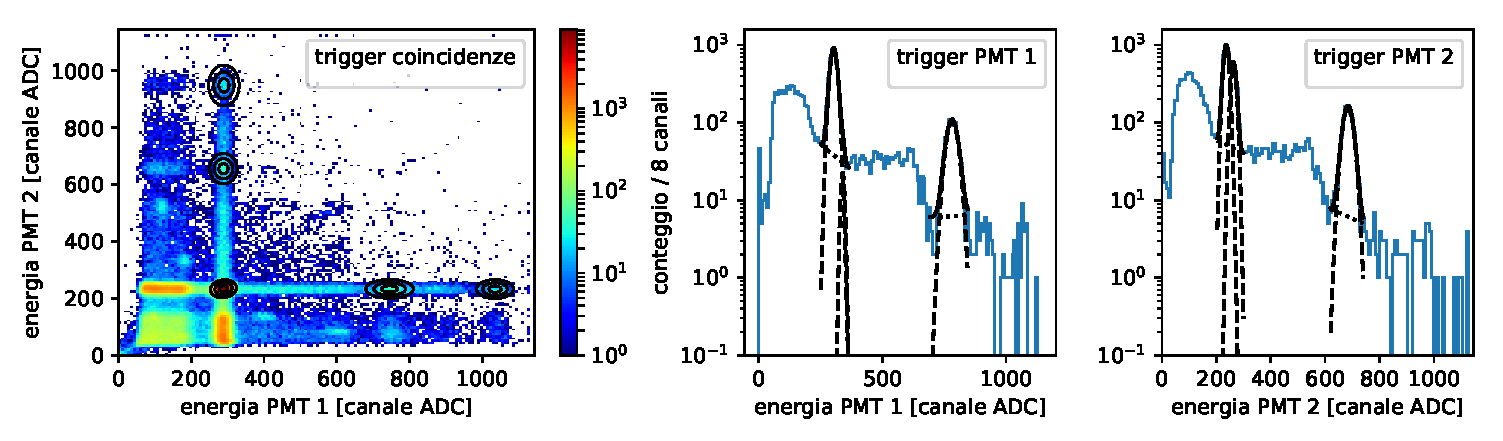
\includegraphics[width=1.5\textwidth]{immagini/ec}
	\caption{\label{fig:ec}
	Dati e fit dei picchi per misurare il braching ratio di cattura elettronica.
	I picchi $\beta_1$ e $\beta_2$ sono fittati con due gaussiane per il problema descritto in \autoref{ref}.
	I risultati dei fit sono in \autoref{tab:fitpicchi}.}
\end{figure}

Questa misura è stata fatta con il circuito A.

\paragraph{Apparato}

Poniamo i due scintillatori allineati uno davanti all'altro usando la guida metallica,
con le facce a distanza \SI{9.0 \pm 0.1}{cm}.
La guida permette di farli scorrere, quindi controlliamo che siano allineati
facendo appoggiare le facce e poi allontanandoli.
Attacchiamo un righello da uno scintillatore all'altro per posizionare la sorgente al centro.
Attacchiamo la sorgente a un supporto che possiamo far scorrere fino ad appoggiarlo ai rivelatori
per controllare che sia allineata al centro.
Controlliamo gli allineamenti con foto da varie angolazioni.

\paragraph{Accettanze}

L'accettanza non è ben definita perché gli scintillatori non sono tronchi di corone sferiche.
Per tenerne conto calcoliamo l'accettanza dall'area sottesa dalla circonferenza dello scintillatore
a 1/3 e 2/3 della profondità, prendiamo la media delle due come accettanza e la differenza come incertezza.
Poiché la sorgente è ben allineata, l'accettanza per le coincidenze a 2 è la stessa.
Risulta $A_1 = A_2 = A_{12} = \num{0.028(12)}$.

\paragraph{Fit dei picchi}

\newcommand*\gauss{\operatorname{gauss}}
\begin{table}
	\hspace{-2em}
	\begin{tabular}{l|l}
		Picco & Modello \\
		\hline
		$\beta_1$, $\beta_2$, $\gamma_1$, $\gamma_2$
		& $Ae^{-\lambda x} + N\gauss(x, \mu, \sigma)$ \\
		$\gamma\beta$, $(\gamma\beta,\beta)$
		& $\big(Ae^{-\lambda x_1} + N\gauss(x_1,\mu_1,\sigma_1)\big)\gauss(x_2,\mu_2,\sigma_2)$ \\
		$\beta\gamma$, $(\beta,\gamma\beta)$
		& $\big(Ae^{-\lambda x_2} + N\gauss(x_2,\mu_2,\sigma_2)\big)\gauss(x_1,\mu_1,\sigma_1)$ \\
		$\beta\beta$
		& $N\gauss(\mathbf x,\boldsymbol\mu,\boldsymbol\Sigma)
		+ A_2e^{-\lambda_2 x_2}\gauss(x_1,\mu_1,\sigma_1)
		+ A_1e^{-\lambda_1 x_1}\gauss(x_2,\mu_2,\sigma_2)$
	\end{tabular}
	\caption{\label{tab:modelli}
	Modelli usati per fittare i vari picchi.
	Con $\gauss(x,\mu,\sigma)$ si intende una gaussiana di media $\mu$ e deviazione standard $\sigma$.
	Le variabili in grassetto sono bidimensionali.
	$\boldsymbol\Sigma$ è la matrice di covarianza.
	Il rate del picco è $N$ moltiplicato per il rate
	e diviso per il numero di eventi registrati dall'ADC e per l'area dei bin.}
\end{table}

\begin{table}
	% tabella generata da ec.py
	\small
	\sisetup{separate-uncertainty=false}
	\hspace{-12em}
	\begin{tabular}{c||ccccc|cc|cc}
		Picco       &     $\beta\beta$ &     $\gamma\beta$ & $\gamma\beta,\beta$ &     $\beta\gamma$ & $\beta,\gamma\beta$ &        $\beta_1$ &      $\gamma_1$ &        $\beta_2$ &      $\gamma_2$ \\ \hline\hline
		$N$         & \num{7.40(5)e+6} &  \num{3.7(12)e+4} &     \num{3.1(9)e+4} &   \num{3.8(7)e+4} &    \num{5.0(15)e+4} & \num{3.02(6)e+4} & \num{5.5(3)e+3} & \num{3.60(7)e+4} & \num{7.0(3)e+3} \\ \hline
		$\mu_1$     &  \num{288.57(5)} &   \num{745.4(28)} &    \num{1035.2(22)} &    \num{288.4(4)} &      \num{289.7(7)} &   \num{303.1(3)} & \num{781.6(11)} &   \num{263.6(7)} &               - \\
		$\sigma_1$  &   \num{11.87(6)} &       \num{22(4)} &         \num{17(3)} &     \num{12.7(4)} &       \num{14.0(8)} &  \num{13.51(29)} &  \num{21.2(11)} &     \num{9.4(5)} &               - \\
		$A_1$       &    \num{123(23)} &       \num{17(4)} &          \num{6(4)} &                 - &                   - &      \num{52(5)} &   \num{6.0(22)} &                - &               - \\
		$\lambda_1$ &  \num{-0.009(4)} & \num{-0.0034(28)} &      \num{0(10)e-3} &                 - &                   - & \num{0.0060(19)} &   \num{0(4)e-3} &                - &               - \\ \hline
		$\mu_2$     &  \num{233.89(3)} &    \num{233.2(4)} &      \num{232.7(6)} &   \num{655.8(17)} &     \num{948.7(14)} &     \num{339(5)} &               - &   \num{236.3(5)} &  \num{684.1(7)} \\
		$\sigma_2$  &   \num{10.53(3)} &     \num{10.9(4)} &       \num{11.1(7)} &    \num{17.7(24)} &         \num{24(4)} &       \num{7(4)} &               - &     \num{9.8(4)} &   \num{17.5(7)} \\
		$A_2$       &      \num{53(6)} &                 - &                   - &    \num{13.8(22)} &          \num{2(4)} &                - &               - &      \num{59(8)} &   \num{7.7(20)} \\
		$\lambda_2$ & \num{0.0148(28)} &                 - &                   - & \num{-0.0014(24)} &     \num{0.013(24)} &                - &               - & \num{0.0039(20)} &  \num{0.004(5)} \\ \hline
		corr.       &   \num{0.098(3)} &                 - &                   - &                 - &                   - &                - &               - &                - &               - \\ \hline
		$\chi^2$    &             87.3 &              54.5 &                40.1 &              74.6 &                44.9 &              2.5 &             7.4 &              0.9 &             6.1 \\
		dof         &               61 &                60 &                  32 &                62 &                  52 &                7 &              11 &                5 &              10
	\end{tabular}
	\caption{\label{tab:fitpicchi}
	Risultati dei fit dei picchi per la misura di branching ratio della cattura elettronica.
	I parametri sono spiegati nella \autoref{tab:modelli}.
	Per $\beta_1$ e $\beta_2$, per compattezza,
	$\mu$ e $\sigma$ del picco più a destra
	(vedi \autoref{fig:ec})
	sono riportate nella casella dell'altro PMT
	e $N$ è la somma delle due normalizzazioni.}
	\sisetup{separate-uncertainty=true}
\end{table}

Poiché, come si vede in \autoref{fig:ec},
tutti i picchi hanno un fondo significativo,
ricaviamo il rate dei picchi fittandoli con gaussiane più fondo.
I fit sono ai minimi quadrati sugli istogrammi.
Riportiamo i modelli usati in \autoref{tab:modelli}
e i risultati dei fit in \autoref{tab:fitpicchi}.

\marginpar{Non si capisce un cazzo di quella tabella enorme.
\begin{enumerate}
\item bisogna leggere l'altra tabella per capire
\item la frase della compattezza è incomprensibile
\item non hai accennato a nessun crosstalk
\item non ci sono le unità di misura
\item aggiusta l'altra tabella perché in quella enorme ci sono $\lambda_{1,2}$ e $A_{1,2}$ mentre in quella di spiegazione ci sono solo $A$ e $\lambda$ per i non $\beta\beta$
\item correlazione con chi?
\end{enumerate} }

Per i picchi $\beta_1$ e $\beta_2$ abbiamo fittato con due gaussiane
per il problema descritto in \autoref{ref} dovuto al crosstalk sull'ADC.
I rate ricavati dalle normalizzazioni sono riportati in \autoref{tab:ecfit}.

\paragraph{Fit dei rate e delle probabilità di interazione}

\begin{table}
	% tabella generata da ec.py
	\hspace{-2em}
	\begin{tabular}{ccc|cc}
		Dato & Input & Valore fittato & Parametro & Valore fittato \\
		\hline
		             $R_{\beta\beta}$ &     \num{4099(26)} &     \num{4096(26)} &      $\R p_{\beta12}$ &  \num{4.31(5)e+3} \\
		            $R_{\gamma\beta}$ &        \num{20(6)} &        \num{18(3)} &       $\R p_{\beta1}$ & \num{5.69(12)e+3} \\
		      $R_{\gamma\beta,\beta}$ &        \num{17(5)} &        \num{23(4)} &       $\R p_{\beta2}$ & \num{5.77(11)e+3} \\
		            $R_{\beta\gamma}$ &        \num{21(4)} &        \num{19(3)} &         $p_{\gamma1}$ &   \num{0.0052(9)} \\
		      $R_{\beta,\gamma\beta}$ &        \num{28(8)} &        \num{25(5)} &         $p_{\gamma2}$ &  \num{0.0058(11)} \\
		                $R_{\beta_1}$ & \num{1.106(23)e+4} & \num{1.110(22)e+4} &               $\Rtot$ &   \num{4.0(7)e+5} \\
		               $R_{\gamma_1}$ &  \num{2.02(12)e+3} &  \num{1.99(12)e+3} &   $\R p_{\beta1}\tot$ &  \num{8.2(14)e+3} \\
		                $R_{\beta_2}$ & \num{1.122(21)e+4} & \num{1.124(21)e+4} &     $p_{\gamma1}\tot$ &    \num{0.024(6)} \\
		               $R_{\gamma_2}$ &  \num{2.17(10)e+3} &   \num{2.19(9)e+3} &   $\R p_{\beta2}\tot$ & \num{1.16(18)e+4} \\
		  $p_{\beta1}\tot/p_{\beta1}$ &       \num{2.0(3)} &     \num{1.44(23)} &     $p_{\gamma2}\tot$ &    \num{0.026(7)} \\
		$p_{\gamma1}\tot/p_{\gamma1}$ &       \num{4.5(8)} &       \num{4.5(8)} &  $\R p_{\beta12}\tot$ &   \num{8.2(8)e+3} \\
		  $p_{\beta2}\tot/p_{\beta2}$ &       \num{2.0(3)} &       \num{2.0(3)} &  & \\
		$p_{\gamma2}\tot/p_{\gamma2}$ &       \num{4.5(8)} &       \num{4.5(8)} &  & \\
		$p_{\beta12}\tot/p_{\beta12}$ &       \num{3.0(4)} &     \num{1.90(18)} &  &
	\end{tabular}
	\caption{\label{tab:ecfit}
	Dati e risultati del fit dei rate e delle probabilità di interazione.
	I rate sono in \si{s^{-1}}.
	$\chi^2/\text{dof} = 2.8$, $\text{dof}=3$, $p=0.04$.
	I ``valori fittati'' dei dati sono il risultato del modello usando i parametri fittati,
	l'unica discrepanza (leggera) con i dati è in $p_{\beta12}\tot/p_{\beta12}$.
	Notiamo che sono compatibili a coppie:
	$R_{\beta1}$ con $R_{\beta2}$,
	$R_{\gamma1}$ con $R_{\gamma2}$,
	$R_{\gamma\beta}$ con $R_{\beta\gamma}$,
	$R_{\gamma\beta,\beta}$ con $R_{\beta,\gamma\beta}$.
	Ci aspettiamo questa compatibilità vista l'elevata simmetria dell'apparato.} 
\end{table}

Impostiamo un fit ai minimi quadrati
in cui i dati sono i rate dei picchi e i rapporti $p_{\dots}/p_{\dots}\tot$ (vedi \autoref{sec:ptotp}),
mentre il modello è dato dalle equazioni in \autoref{sec:eqrate}.
I risultati dettagliati del fit sono riportati in \autoref{tab:ecfit}.
I risultati importanti per la misura di cattura elettronica sono
\begin{align*}
	\R
	&= (2.7 \pm 1.1) \cdot 10^5 \,\si{s^{-1}} = \\
	&= \left(2.68
	\pm 1.12^\text{(accettanze)}
	\pm 0.08^\text{(statistico)}
	\pm 0.00^\text{(rapporti)}\right) \cdot 10^5 \,\si{s^{-1}}, \\
	\Rtot
	&= (4.0 \pm 0.7) \cdot 10^5 \,\si{s^{-1}} = \\
	&= \left(3.98
	\pm 0.66^\text{(statistico)}
	\pm 0.16^\text{(rapporti)}\right) \cdot 10^5 \,\si{s^{-1}}, \\
	\R/\Rtot
	&= 0.67 \pm 0.30 = \\
	&= 0.67 \pm 0.28^\text{(accettanze)} \pm 0.11^\text{(statistico)} \pm 0.03^\text{(rapporti)}.
\end{align*}
Nel calcolo di $\R/\Rtot$ abbiamo tenuto conto della correlazione tra $\R$ e $\Rtot$,
che però è praticamente trascurabile (\SI{0.2}\%).
$\R/\Rtot$ è compatibile con il valore noto 0.9
ma ha un'incertezza del \SI{50}\% data dall'incertezza sull'accettanza,
ovvero dal non aver usato un modello preciso per la probabilità di interazione con il rivelatore.

